\chapter{Implementace}\label{implementation}

V této kapitole se budu věnovat převážně některým obecným součástem aplikace a jak jsem došel k jejich výsledné podobě. Obsahem \emph{není} popis realizace funkčních požadavků aplikace, přestože jsem jejich implementací strávil nezanedbatelné množství času. Tento popis je již totiž dostupný ve formě analýzy a návrhu, kterým odpovídá.\\

%%%%%%%%%%%%%%%%%%%%%%%%%%%%%%%%%%%%%%%%%%%%%%%%%%%%%%%%%%%%%%%%%%%%%%%%%%%%%%%%
%%%%%%%%%%%%%%%%%%%%%%%%%%%%%%%%%%%%%%%%%%%%%%%%%%%%%%%%%%%%%%%%%%%%%%%%%%%%%%%%
%%%%%%%%%%%%%%%%%%%%%%%%%%%%%%%%%%%%%%%%%%%%%%%%%%%%%%%%%%%%%%%%%%%%%%%%%%%%%%%%
%%%%%%%%%%%%%%%%%%%%%%%%%%%%%%%%%%%%%%%%%%%%%%%%%%%%%%%%%%%%%%%%%%%%%%%%%%%%%%%%

\section{Podpůrné nástroje vývoje}

\subsection{Webpack}

Webpack \cite{webpack} je software, který zpracovává součásti webových aplikací a tvoří z nich balíčky vhodné pro webové prohlížeče. Primárně je zaměřen na Javascript, ale dokáže zpracovávat i řadu dalších formátů, přes styly v css, sass či stylus, obrázky v png, jpg, svg, ale také konfigurace v json, yaml a dalších.\\
Hlavním důvodem, proč používat Webpack, je možnost rozdělování kódu do jednotlivých souborů. Při programování je pohodlné mít oddělené ucelené komponenty, různé konfigurační soubory apod. Výstupem webpacku jsou poté typicky pouze čtyři soubory: dva obsahující logiku aplikace (.js) a dva pro stylování (.css), přičemž logika i styly jsou rozděleny na samotnou aplikaci - kód programátora, a kód třetích stran - tzv. \code{vendor}.

\paragraph{Použití loaderů.} Další příležitost k použití Webpacku přichází ve chvíli, kdy chceme v projektu mít kód, který není v cílovém prohlížeči podporován. Tím může být například SASS, nebo třeba i moderní syntaxe Javascriptu řídící se standardem ES6 či novějším. S pomocí Webpacku lze nastavit, aby se při zpracování některých souborů použil \emph{loader}, který například převede SASS na CSS, konstrukce ES6 na ES5 apod. \cite{webpack-ackee}.

\paragraph{Webpack ve spolupráci s Vue.js.} Konfigurace Webpacku může být pro neznalého uživatele až příliš obsáhlá a může být jednoduché v ní udělat chybu, kvůli které bude například výsledný build aplikace neoptimalizovaný a tudíž pomalý. Vývojáři Vue tento problém mitigovali tak, že celá optimalizovaná konfigurace Webpacku je součástí \code{vue-cli}, což znamená, že stačí mít v projektu jako závislosti právě tento npm modul, a pokud nejsou vyžadovány žádné pokročilé funkce, funguje vše \emph{automagicky}\footnote{Nejedná se o překlep, jde o spojení slov automaticky a magicky}. Pro účely porovnání jsem se podíval, jak dlouhá je konfigurace webpacku, kterou má Vue automaticky v sobě - jedná se o \emph{1490 řádků kódu}.

%%%%%%%%%%%%%%%%%%%%%%%%%%%%%%%%%%%%%%%%
%%%%%%%%%%%%%%%%%%%%%%%%%%%%%%%%%%%%%%%%

\subsection{Vue-UI}

V předchozím paragrafu jsem popisoval výhodu použití Vue-CLI, ke kterému je ale vhodné říci i několik dalších slov, jelikož se jedná o velmi prakticky nástroj, usnadňující mnoho běžných požadavků na správu projektu.\\
Zaměřit bych se chtěl především na možnost spuštění grafického prostředí, pomocí příkazu \code{vue ui} z terminálu, které si vytvoří vlastní webový server a na adrese \code{localhost:8000} spustí grafickou správu projektu. Ta obsahuje následující možnosti:
\begin{itemize}
    \item \emph{přehled projektů}, který nabízí rychlou kontrolu dostupných aktualizací použitých balíčků, kontrolu bezpečnostních mezer nebo RSS čtečku novinek od Vue komunity,
    \item \emph{instalované pluginy}, což jsou běžné npm balíčky, ke kterým je ale možné přidat další konfiguraci. Jedná se například o pluginy pro samotné \code{vue-cli}, \code{eslint} nebo třeba knihovnu \code{vuetify}, která poskytuje grafické komponenty, a pomocí tohoto pluginu vkládá do výsledného buildu pouze ty, které jsou skutečně v aplikaci používány.
    \item \emph{instalované závislosti}, u kterých je možné jednoduše hromadně aktualizovat na nové verze, zobrazovat, jakou verzi používáme a jaká je nejnovější, nebo přes jednotné hledání instalovat nové závislosti,
    \item \emph{úlohy spouštěné nad kódem aplikace}, asi nejpraktičtější součást Vue-UI, ze které je možné spouštět lokální dev-server ale také build pro produkci. Největší výhodou spouštění těchto úloh z UI je ta, že po skončení úlohy jsou zde dostupné bohaté informace o velikosti výsledných souborů a přehled, jak velká je která závislost. Jako příklad uvedu dále optimalizaci velikosti překladů.
\end{itemize}

\begin{figure}[h]
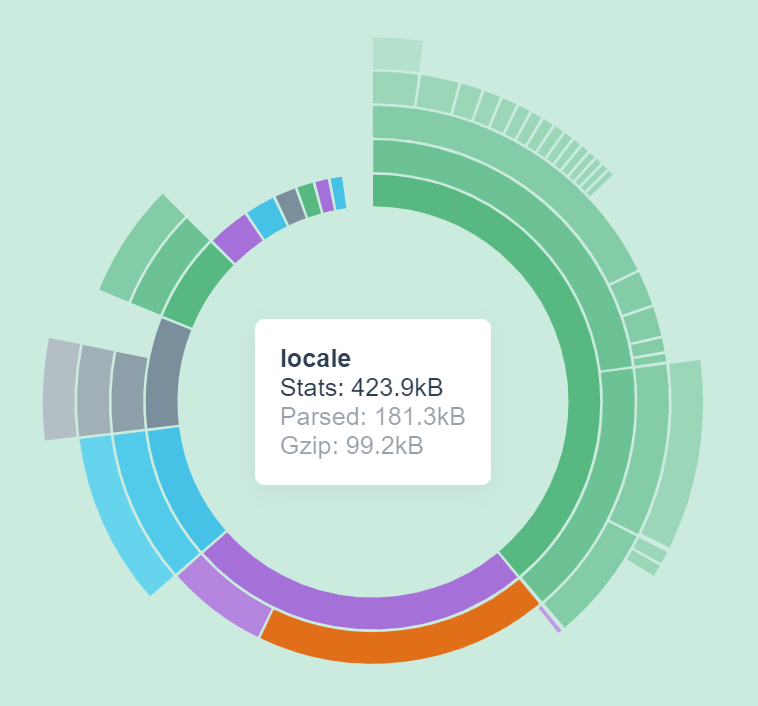
\includegraphics[width=0.6\textwidth]{../png/cli/analyze-moment.png}
\caption[Analýza velikosti výsledné aplikace: překlady moment.js]{Analýza velikosti výsledné aplikace: překlady moment.js (na obrázku popsáno jako locale a označeno oranžově) zabírají velké procento z celkové velikosti souboru.} \label{picture:cli:analyze}
\end{figure}

\paragraph{Optimalizace velikosti aplikace odebráním zbytečných překladů.} Jednou ze závislostí, kterou v projektu používám, je knihovna \emph{moment} \cite{momentjs}, která se stará o parsování a zobrazování data a času, a jejíž součástí jsou i překlady do 127 jazyků. Jeden soubor s jazykem má sice \uv{pouze} 172 řádků kódu, ale při vzájemném pronásobení to už je \emph{21844 řádků}. Není tak divu, že při analýze velikostu výsledných souborů pomocí Vue-UI jsem odhalil, že tyto překlady zabírají téměř \emph{15\% celkové velikosti} souboru s kódem třetích stran (\code{vendor}), jak je znázorněno na obrázku \ref{picture:cli:analyze}.

Našel jsem si tedy řešení spočívající v přidání jednoho řádku konfigurace \cite{momentjs-ignore-locale}, jehož cílem je nezahrnovat do výsledného buildu ty jazyky, které nepoužívám (což jsou všechny kromě češtiny a angličtiny). Výsledek je takový, že nyní překlady nezabírají \emph{ani jedno celé procento}.

%%%%%%%%%%%%%%%%%%%%%%%%%%%%%%%%%%%%%%%%%%%%%%%%%%%%%%%%%%%%%%%%%%%%%%%%%%%%%%%%
%%%%%%%%%%%%%%%%%%%%%%%%%%%%%%%%%%%%%%%%%%%%%%%%%%%%%%%%%%%%%%%%%%%%%%%%%%%%%%%%
%%%%%%%%%%%%%%%%%%%%%%%%%%%%%%%%%%%%%%%%%%%%%%%%%%%%%%%%%%%%%%%%%%%%%%%%%%%%%%%%
%%%%%%%%%%%%%%%%%%%%%%%%%%%%%%%%%%%%%%%%%%%%%%%%%%%%%%%%%%%%%%%%%%%%%%%%%%%%%%%%

\section{Router}

\begin{figure}[h]
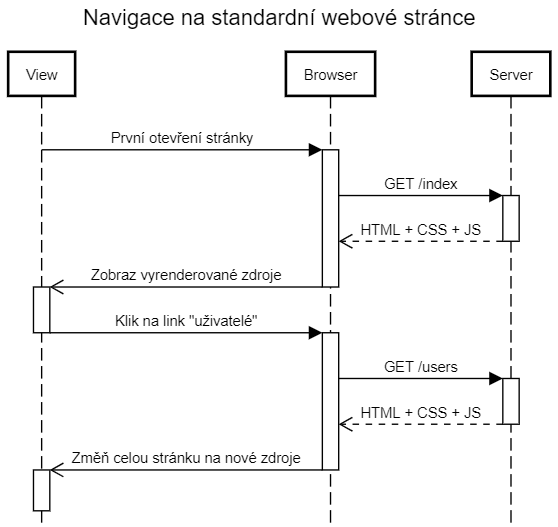
\includegraphics[width=0.7\textwidth]{../png/diagrams/sequence-http-navigate.png}
\caption[Sekvenční diagram navigace na standardní webové stránce]{Sekvenční diagram navigace na standardní webové stránce: Pro každý link existuje cesta na serveru, který odpovídá kompletním obsahem této stránky.} \label{picture:route:http}
\end{figure}

Jednou z prvních komponent, kterou jsem k čistému Vue.js přidal, byl oficiální Vue Router \cite{vue-router}. Koncept routeru je dobře znám z jakékoliv jiné aplikace, která nějak pracuje s prohlížečem uživatele.\\
Rozdíl Vue.js routeru oproti tomu, který je používán třeba v PHP, spočívá v dynamičnosti celého javascriptového frameworku: oproti standardním webovým stránkám, kde přesměrování na novou adresu skutečně vyvolá požadavek na server, který odpoví obsahem stránky na dané URL (diagram \ref{picture:route:http}), zde se vše děje dynamicky přímo na klientském zařízení, obsah je vyměněn pomocí Javascriptu a hodnota adresního řádku se změní pouze \uv{pro efekt} - tj. aby uživatel věděl, kde se nachází, a aby mohl adresu zkopírovat a sdílet. Samozřejmě i zde většinou dochází k načítání dat nově otevřené stránky, ale vše je typicky asynchronní - stránka se změní ihned a teprve poté jsou do ní doplněna data - viz diagram \ref{picture:route:vue}.

\begin{figure}[h]
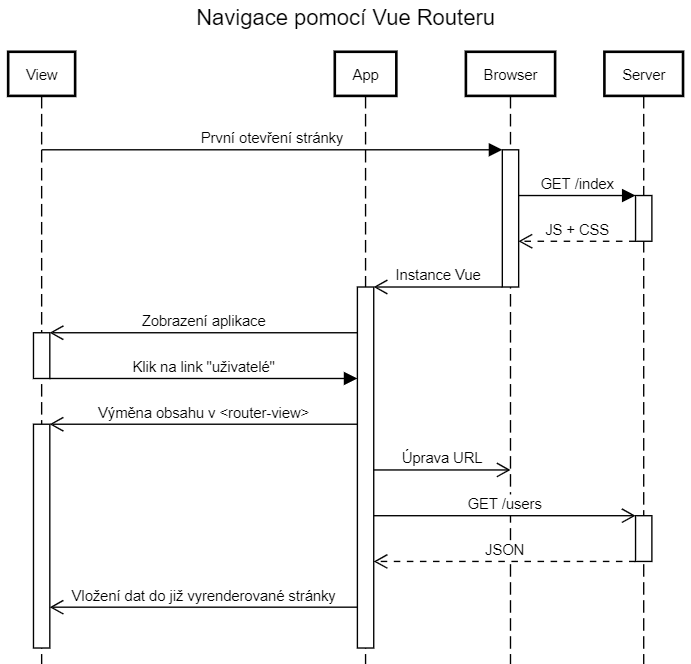
\includegraphics[width=0.9\textwidth]{../png/diagrams/sequence-vue-router.png}
\caption[Sekvenční diagram navigace v aplikaci pomocí Vue Router]{Sekvenční diagram navigace v aplikaci pomocí Vue Router: Kompletní obsah aplikace se ze serveru stáhne pouze při prvním přístupu, navigaci v aplikaci řeší Vue Router přímo na klientu a od serveru či jiného API vyžaduje pouze konkrétní data, která v aplikaci zobrazuje.} \label{picture:route:vue}
\end{figure}

% title Navigace na standardní webové stránce

% View->Browser:První otevření stránky
% activate Browser
% Browser->Server:GET /index
% activate Server
% Server-->>Browser:HTML + CSS + JS
% deactivate Server
% Browser->>View:Zobraz vyrenderované zdroje
% deactivate Browser
% activate View


% View->Browser:Klik na link "uživatelé"
% deactivate View
% activate Browser
% Browser->Server:GET /users
% activate Server
% Server-->>Browser:HTML + CSS + JS
% deactivate Server
% Browser->>View:Změň celou stránku na nové zdroje
% deactivate Browser
% activate View


% title Navigace pomocí Vue Routeru
% 
% participant View
% participant App
% participant Browser
% participant Server
% 
% View->Browser:První otevření stránky
% activate Browser
% Browser->Server:GET /index
% activate Server
% Server-->>Browser:JS + CSS
% deactivate Server
% Browser->>App:Instance Vue
% deactivate Browser
% activate App
% App->>View:Zobrazení aplikace
% activate View
% 
% 
% View->App:Klik na link "uživatelé"
% deactivate View
% App->>View:Výměna obsahu v <router-view>
% activate View
% App->>Browser:Úprava URL
% App->>Server:GET /users
% activate Server
% Server-->>App:JSON
% deactivate Server
% App->>View:Vložení dat do již vyrenderované stránky
% 

\paragraph{Titulky stránek.} Lehce matoucí může u tohoto \emph{frontendového routování} být nastavování titulků stránek, tedy \code{<title>} tagů v HTML. Celá aplikace má totiž stále pouze jeden \code{<title>} zapsaný v souboru \code{index.html}, který se sám o sobě při navigaci za pomocí routeru vůbec nemění. K vyřešení tohoto problému sice ve Vue Routeru neexistuje nativní podpora, ale řešení je opravdu snadné - je popsáno v jednom z \emph{issues} v repozitáři na GitHubu \cite{vue-router-title} a spočívá v doplnění titulků do \code{meta} atributů cest, viz ukázka kódu \ref{code:vue-router-title1}, a dále úpravě samotné instance routeru, viz ukázka kódu \ref{code:vue-router-title2}.

\begin{listing}[]
\begin{minted}[linenos,frame=lines]{javascript}
{
    path: '/',
    component: Homepage,
    meta: {
        title: 'Swordfish'
    }
}
\end{minted}
\caption{Nastavování titulků stránek pomocí Vue routeru - úprava definic} \label{code:vue-router-title1}
\end{listing}

\begin{listing}[]
    \begin{minted}[linenos,frame=lines]{javascript}
router.beforeEach((to, from, next) => {
    document.title = to.meta.title;
    next();
})
\end{minted}
\caption{Nastavování titulků stránek pomocí Vue routeru - úprava instance routeru} \label{code:vue-router-title2}
\end{listing}

Toto nastavování titulků stránek jsem nakonec ještě více upravil po svém, jelikož jsem chtěl mít v titulcích i konkrétní hodnoty, které se zobrazují na dané stránce - například při úpravě skladu \emph{Centrální sklad Praha} nechci mít v titulku \uv{Úprava skladu}, ale \uv{Úprava skladu 'Centrální sklad Praha'}. Jelikož jsou ale tyto informace načítány dynamicky až po vstupu na danou stránku (URL stránky může být například \code{/stocks/12/edit} - z té to tedy vyčíst nelze), je nutné i titulek nastavovat dynamicky. Zachoval jsem tedy jako výchozí hodnotu titulku stránky ten, který je nastaven přímo v definici cesty v routeru (ukázka kódu \ref{code:vue-router-title1}), avšak zevnitř komponenty je možné pomocí jednotné funkce titulek obohatit dalšími informacemi - jako například názvem upravované položky.

\paragraph{Drobečková navigace.} Další úpravou routeru, kterou jsem do jisté míry realizoval po svém, je generování drobečkové navigace. Vue Router ve spojení s Vuetify nemají nativní podporu pro zjišťování rodičovských stránek, a tak jsem si lehkou úpravou a vlastní komponentou pro vykreslování \emph{Breadcrumbs} toto zautomatizoval:\\
Každá definovaná routa má nastaveného rodiče, ke kterému poskytuje \emph{getter}. Ve vykreslování drobečkové navigace se poté na aktuální routě zjišťují rekurzivně její rodiče, a včetně jejich parametrů se z nich zpětně tvoří celý strom navigace.\\
Co se na první pohled může zdát jednoduché, se zkomplikuje ve chvíli, kdy chceme mít v cestě parametrizovanou stránku.\\
Například v URL \code{/stocks/1/locations/12/update} je potřeba v definici routy nahradit všechny identifikátory jejich reálnými hodnotami, které ale naštěstí Vue Router poskytuje i během runtime. Funkce pro vytvoření jednoho odkazu, ze kterých se skládá drobečková navigace, je znázorněna v ukázce kódu \ref{code:router:buildPath} - jejími argumenty jsou definice cesty v routě a objekt s aktuálními hodnotami parametrů.

\begin{listing}[H]
    \begin{minted}[linenos,frame=lines]{javascript}
function buildPath(pathWithPlaceholders, parameters) {
    let routePath = pathWithPlaceholders.replace(/\([^/]+\)/g, '');
    const matches = routePath.match(/(:[a-zA-Z]+\/)|(:[a-zA-Z]+$)/g);
    if (matches !== null) {
        for (const match of matches) {
            const matchParam = match.replace(/\//, '').replace(/:/, '');
            routePath = routePath
                        .replace(match, parameters[matchParam] + '/');
        }
    }
    return routePath;
}
\end{minted}
\caption[Automatické generování drobečkové navigace]{Automatické generování drobečkové navigace z definic Vue Routeru, včetně podpory parametrizovaných zanořených cest} \label{code:router:buildPath}
\end{listing}

%%%%%%%%%%%%%%%%%%%%%%%%%%%%%%%%%%%%%%%%%%%%%%%%%%%%%%%%%%%%%%%%%%%%%%%%%%%%%%%%
%%%%%%%%%%%%%%%%%%%%%%%%%%%%%%%%%%%%%%%%%%%%%%%%%%%%%%%%%%%%%%%%%%%%%%%%%%%%%%%%
%%%%%%%%%%%%%%%%%%%%%%%%%%%%%%%%%%%%%%%%%%%%%%%%%%%%%%%%%%%%%%%%%%%%%%%%%%%%%%%%
%%%%%%%%%%%%%%%%%%%%%%%%%%%%%%%%%%%%%%%%%%%%%%%%%%%%%%%%%%%%%%%%%%%%%%%%%%%%%%%%

\section{Moderní webová aplikace}

V kapitole \ref{technology} jsem zmiňoval, že skladník bude aplikaci používat z nativní Android aplikace, která bude obalovat WebView, a vedoucí skladu si aplikaci otevře v běžném browseru - pro obě použití by níže popisovaná konfigurace nebyla potřeba, avšak pokud by někdo nepotřeboval čtečku čárových kódů - což je jediný důvod, proč skladníci používají jako základ nativní Android aplikaci - je možné si otevřít na mobilu běžnou stránku a použít volbu \uv{Přidat na plochu}. Tím vznikne zástupce, který zobrazuje \emph{favicon} webové stránky a po jehož otevření se opět otevře běžný webový prohlížeč.\\
Pokud je však na stránce definovaný \code{manifest.json} pro webové aplikace, může se po otevření tohoto zástupce otevřít stránka v režimu celé obrazovky, a to případně i se skrytými ovládacími prvky - vše tak vypadá, jako kdyby se jednalo o nativní nainstalovanou aplikaci. Základní konfigurace tohoto manifestu je vidět v ukázce kódu \ref{code:webapp-manifest}.

\begin{listing}[H]
\begin{minted}[linenos,frame=lines]{json}
{
  "name": "Swordfish",
  "icons": [
    {
      "src": "favicon/swordfish-192x192.png",
      "sizes": "192x192",
      "type": "image/png"
    },
    {
      "src": "favicon/swordfish-512x512.png",
      "sizes": "512x512",
      "type": "image/png"
    }
  ],
  "start_url": "/",
  "display": "standalone",
  "orientation": "portrait",
  "background_color": "#009688"
}

\end{minted}
\caption{Manifest pro webové aplikace} \label{code:webapp-manifest}
\end{listing}

Tento soubor je vlastně také první krok k vytvoření PWA - Progresivní webové aplikace, což znamená takové webové aplikace, která do jisté míry může fungovat i bez připojení k internetu. Využívá k tomu Service Worker API \cite{service-worker-api}, jehož specifikace je v době psaní tohoto textu stále ve stavu návrhu, přestože vzniká již od května roku 2014 \cite{service-worker-first}.\\
I přes nedokončenou speficikaci se již PWA běžně používají a i ve skladové aplikaci by bylo vhodné toto API využít, to již ale není předmětem této práce a proto jej v tuto chvíli dále nerozvádím.

%%%%%%%%%%%%%%%%%%%%%%%%%%%%%%%%%%%%%%%%%%%%%%%%%%%%%%%%%%%%%%%%%%%%%%%%%%%%%%%%
%%%%%%%%%%%%%%%%%%%%%%%%%%%%%%%%%%%%%%%%%%%%%%%%%%%%%%%%%%%%%%%%%%%%%%%%%%%%%%%%
%%%%%%%%%%%%%%%%%%%%%%%%%%%%%%%%%%%%%%%%%%%%%%%%%%%%%%%%%%%%%%%%%%%%%%%%%%%%%%%%
%%%%%%%%%%%%%%%%%%%%%%%%%%%%%%%%%%%%%%%%%%%%%%%%%%%%%%%%%%%%%%%%%%%%%%%%%%%%%%%%

\section{Překlady}

Novou aplikaci je dnes vhodné hned od počátku psát jako \emph{multijazyčnou} - jako základ tedy například v češtině a angličtině.\\
Pro překlady Vue.js aplikací je vhodné použít knihovnu \code{vue-i18n}\footnote{název je zkratka slova \emph{internationalization} - číslovka 18 značí počet přeskočených znaků} \cite{vue-i18n}, jejíž použití je obdobné, jako známe z jiných jazyků. Zatímco například v PHP se často překlady zapisují do \code{.yaml} nebo \code{.neon}, což jsou formáty, které sice umožňují například zanořování, ale s dalšími funkcemi už si často neporadí, zde se texty zapisují do běžného \code{.js} souboru (ukázka kódu \ref{code:i18n-def}), jehož výstupem je JSON. To znamená, že můžeme používat libovolné konstrukce Javascriptu, od standarního zápisu (klíč \code{close} ve zmiňované ukázce), přes spojování řetězců a používání konstant (podklíče \code{user}), po proměnné klíče (podklíče \code{orderState}), jejichž definice se doplní z číselníku načteného klidně i z jiného souboru. Kreativní autor překladů by jistě našel i prostor pro použití cyklů nebo funkcí, mně ale pro potřeby skladové aplikace stačily znázorněné možnosti.

\begin{listing}[h]
\begin{minted}[linenos,frame=lines]{js}
const user = "uživatele";

{
    close: "Zavřít",
    user: {
        create: "Vytvořit " + user,
        update: "Upravit " + user
    },
    orderState: {
        [OrderStateEnum.CREATED]: 'Vytvořená',
        [OrderStateEnum.SENT]: 'Odeslaná',
    }
}
\end{minted}
\caption[Definice překladů pro i18n]{Definice překladů pro i18n, včetně pokročilých funkcí jako například spojování řetězců nebo využítí číselníků.} \label{code:i18n-def}
\end{listing}

\paragraph{Překlady a uživatelská nápověda.} Jelikož výsledná aplikace obsahuje i stručnou nápovědu, která má zatím pouze textový obsah, využil jsem pro zápis jejího obsahu také formát, který používá \code{i18n} pro překlady. Tyto texty jsem ale neintegroval do seznamu obecných překladů v aplikaci, nýbrž s nimi pracuji odděleně - pomocí vlastního řešení pro zobrazování nápovědy. Tím mohu všechny texty této \uv{sekce} načíst hromadně a umožnit v nich například vyhledávání, nebo je vkládám přímo k formulářovým atributům, které dokumentují.

%%%%%%%%%%%%%%%%%%%%%%%%%%%%%%%%%%%%%%%%%%%%%%%%%%%%%%%%%%%%%%%%%%%%%%%%%%%%%%%%
%%%%%%%%%%%%%%%%%%%%%%%%%%%%%%%%%%%%%%%%%%%%%%%%%%%%%%%%%%%%%%%%%%%%%%%%%%%%%%%%
%%%%%%%%%%%%%%%%%%%%%%%%%%%%%%%%%%%%%%%%%%%%%%%%%%%%%%%%%%%%%%%%%%%%%%%%%%%%%%%%
%%%%%%%%%%%%%%%%%%%%%%%%%%%%%%%%%%%%%%%%%%%%%%%%%%%%%%%%%%%%%%%%%%%%%%%%%%%%%%%%

\section{State management pattern} \label{impl:vuex}

Jako první se zde sluší říci, co to vlastně \emph{State management pattern} je. Ve Vue.js aplikaci máme typicky velké množství komponent, které mezi sebou často potřebují sdílet nějaký \emph{stav}. Nabízí se tedy vytvoření centrálního bodu, který bude stav udržovat a umožní jej měnit. Na změny by v ideálním případě měly dotčené komponenty reagovat automaticky, a tyto změny by také měly být nějak řízeny, aby nebylo možné nastavit nevalidní hodnoty. Přesně toto nabízí knihovna \emph{Vuex} \cite{vuex}, jejíž interní cyklus popisuje diagram \ref{picture:vuex}.

\begin{figure}[h]
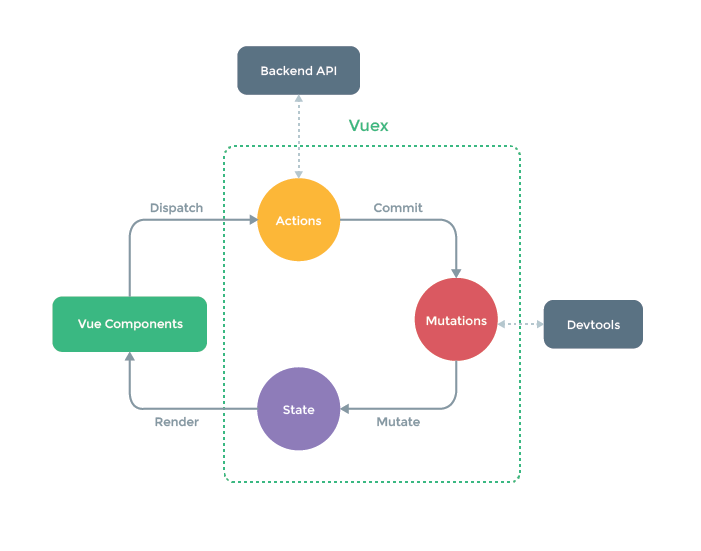
\includegraphics[width=\textwidth]{../png/diagrams/vuex.png}
\caption{Diagram použití Vuex}\label{picture:vuex}
\end{figure}

Nebudu zde rozepisovat detaily jejího použití, ty jsou dostupné kdykoliv online v její kvalitní dokumentaci. Popíšu ale své vlastní zkušenosti s touto knihovnou a jak jsem implementoval některá vylepšení. Začněme však od kraje - jako první jsem Vuex použil pro zobrazování snack message - tedy krátkých informačních zpráv, které se zobrazují uživateli ve spodní části obrazovky, především jako potvrzení jeho akce. K tomu jsem použil Vuex, do jehož stavu jsem ukládal obsah zprávy a případně její trvání. Zaslání takové zprávy znázorňuje ukázka kódu \ref{code:vuex-snack-use}.

\begin{listing}[h]
\begin{minted}[linenos,frame=lines]{js}
this.$store.dispatch('snackbar/setSnack', '<message to display>');
\end{minted}
\caption{Vuex pro snackbar-message: použití z jiné komponenty} \label{code:vuex-snack-use}
\end{listing}

Výše uvedený kód se mi ovšem v průběhu psaní aplikace přestal líbit, neboť zobrazování těchto zpráv je velmi častá operace a její vyvolání není v ukázce příliš jednoduché. Proto jsem si nastudoval mixiny ve Vue.js \cite{vue-mixin} a vytvořil mixin\footnote{Mixin je možné použít pro definici dat a metod, kterými má komponenta disponovat, a které se do ní vloží při jejím vytvoření. Výhodou je, že mixin je znovupoužitelný a může být vložen do libovolného počtu komponent.}, který zjednodušuje zasílání zpráv do Snackbaru. Použití v komponentě vybavené takovým mixinem je znázorněné na ukázce kódu \ref{code:snack-mixin}.

\begin{listing}[h]
\begin{minted}[linenos,frame=lines]{js}
this.snack('<message to display>');
\end{minted}
\caption{Použití mixinu pro zjednodušení zasílání zpráv do Snackbaru} \label{code:snack-mixin}
\end{listing}

\paragraph{Persistentní úložiště.} Když už máme efektivně vyřešené, jak data ukládáme, a aby se neměnila \emph{jen tak}, ale vždy řízeně, může být v některých případech škoda, že v javascriptovém frameworku stačí jedno obnovení stránky pomocí \code{F5}, \code{ctrl-r} či chcete-li tlačítkem v prohlížeči, a všechna tato data se ztratí, neboť bylo vše uloženo pouze v paměti stránky, která se touto akcí celá přepíše. I v aplikaci pro správu skladu jsem se dostal k tomu, že některé věci bych potřeboval uložit tak, aby se nepřemazaly. Projdu nyní jednotlivé moduly, které ve Vuex v době psaní tohoto textu používám, a okomentuji jejich možnosti persistence:

\begin{itemize}
    \item \emph{Stav připojení k API:} modul udržující informaci, zda je dostupné API backendové části aplikace.
        \begin{itemize}
            \item Ukládání tohoto modulu persistentně nemá příliš smysl, protože drží vždy pouze aktuální informaci.
        \end{itemize}
    \item \emph{Loader:} tedy ukazatel, že se něco stahuje. V aplikaci rozlišuji dva typy loaderů: jeden nenápadný ve spodní části obrazovky, a druhý znemožňující provádět jakékoliv akce, dokud se obsah nenačte. U prvního zmiňovaného je navyšován počet požadavků, které běží, a teprve při doběhnutí všech se loader skryje.
        \begin{itemize}
            \item Vzhledem k možnému vyššímu počtu běžících požadavků se nabízí, že by tato data mohla být persistentní, ale ve výsledku je to také nevhodné, protože při obnovení stránky se všechny běžící požadavky zahodí, a jejich potenciální výsledek je ignorován.
        \end{itemize}
    \item \emph{Cache:} místní úložiště dat z API
        \begin{itemize}
            \item Tato část úložiště je detailněji popsána v sekci \ref{impl:cache} níže.
        \end{itemize}
    \item \emph{Autorizace:} Jelikož se uživatelé do aplikace přihlašují, a backendové API je samozřejmě zabezpečené proti neoprávněnému přístupu, je potřeba na klientském zařízení udržovat informace o přihlášení. Aplikace implementuje protokol OAuth2 \cite{oauth2rfc}, který na klientském zařízení pracuje s dočasnými identifikátory \code{access\_token} a \code{refresh\_token} plus některými dalšími položkami, tyto dvě jsou ale nejkritičtější. Ukládání těchto tokenů by se teoreticky mohlo hodit, aby se uživatel nemusel při znovunačtení stránky znovu přihlašovat.
        \begin{itemize}
            \item Jelikož znalost tokenu prakticky opravňuje kohokoliv vystupovat pod jménem uživatele, který token při přihlášení získal, nesmí být ani jeden z nich ukládán kamkoliv jinam než do aplikace samotné. Z toho důvodu není doporučováno ukládat tokeny persistentně, existuje však zde jedna výjimka. Během vývojového procesu, pokud se pracuje s API, které je zabezpečené, používáme tyto tokeny také. V takovém případě je možné tokeny ukládat persistentně, protože s nimi pracuje pouze vývojář, který používá testovací uživatele a testovací data - nehrozí tedy žádný únik či poškození dat reálných uživatelů.
        \end{itemize}
    \item \emph{Snackbar:} modul pro zobrazování krátkých zpráv uživateli.
        \begin{itemize}
            \item Z logiky věci zde vyplývá, že nemá smysl po přenačtení stránky zobrazovat stále stejnou jednorázovou zprávu, modul tedy není nastaven jako persistentní.
        \end{itemize}
    \item \emph{Záznam času stráveného plněním úkolu:} tento modul ukládá, kdy bylo spuštěno měření času stráveného plněním úkolu a další spjaté informace.
        \begin{itemize}
            \item Tuto informaci je naopak velmi důležité ukládat persistentně, neboť při přenačtení stránky je důležité, aby čas nebyl resetován.
        \end{itemize}
    \item \emph{Uživatelská konfigurace aplikace:} zde jsou uloženy informace jako například jazyk, tmavý režim, povolení záznamu času apod.
        \begin{itemize}
            \item Tyto informace bych rád ukládal na API, avšak to zatím takové položky nepodporuje. Proto je také ukládám lokálně a modul je tedy persistentní.
        \end{itemize}
\end{itemize}

Obsah těch modulů, které jsem vyhodnotil jako vhodné k persistenci, ukládám pomocí vlastního řešení do \emph{LocalStorage} webového prohlížeče. V definici modulu pro to stačí nastavit příznak \code{persistent}, případně \code{devPersistent} pro ukládání pouze ve vývojovém režimu, a o zbytek se postará můj globální handler nastavený pro všechny akce Vuex - který při zapnutí aplikace existující stav načte a jakoukoliv změnu zapíše právě i do \emph{LocalStorage}.

%%%%%%%%%%%%%%%%%%%%%%%%%%%%%%%%%%%%%%%%%%%%%%%%%%%%%%%%%%%%%%%%%%%%%%%%%%%%%%%%
%%%%%%%%%%%%%%%%%%%%%%%%%%%%%%%%%%%%%%%%%%%%%%%%%%%%%%%%%%%%%%%%%%%%%%%%%%%%%%%%
%%%%%%%%%%%%%%%%%%%%%%%%%%%%%%%%%%%%%%%%%%%%%%%%%%%%%%%%%%%%%%%%%%%%%%%%%%%%%%%%
%%%%%%%%%%%%%%%%%%%%%%%%%%%%%%%%%%%%%%%%%%%%%%%%%%%%%%%%%%%%%%%%%%%%%%%%%%%%%%%%

\section{Hlídání konektivity}

V moderních aplikacích, které veškerá data ukládají na API, je vhodné hlídat dostupnost tohoto API.\\
Prvním krokem k realizaci této funkčnosti bylo zjišťovat aktuální stav připojení - tedy zda je aplikace online, nebo offline. Jako první jsem našel vlastnost prohlížeče \code{window.navigator.onLine} \cite{online}, která by přesně o tomto měla informovat a navíc poskytuje i možnosti poslouchat její změny pomocí běžných JS eventů.\\
Po hlubším prozkoumání jsem ale zjistil, že tento stav odpovídá pouze dostupnosti \emph{místní sítě}, tj. například dostupnost nejbližšího routeru. Pokud bude fungovat spojení mezi prohlížečem a routerem, ale router samotný nebude mít přístup k internetu, bude tento stav mít hodnotu \code{true}, což ale už pro mé potřeby není vhodné - potřebuji znát dostupnost backendového API.\\
Po tomto zjištění jsem tedy připravil vlastní řešení, které periodicky zasílá dotazy na výchozí endpoint API, ve kterém kontroluje pouze návratový kód. Kontrola probíhá v minutových intervalech a při odpojení od sítě častěji. Při zaimplementování tohoto řešení mě napadlo, zda nebude problém s tím, že by funkce využívala zbytečně moc dat, provedl jsem proto zběžné výpočty: Velikost jednoho požadavku pro zjištění konektivity je 280 B. Při jednom požadavku za minutu to dělá 16.8 kB za hodinu, což je za osmihodinovou směnu 134,4 kB - tedy zcela zanedbatelná velikost.

%%%%%%%%%%%%%%%%%%%%%%%%%%%%%%%%%%%%%%%%%%%%%%%%%%%%%%%%%%%%%%%%%%%%%%%%%%%%%%%%
%%%%%%%%%%%%%%%%%%%%%%%%%%%%%%%%%%%%%%%%%%%%%%%%%%%%%%%%%%%%%%%%%%%%%%%%%%%%%%%%
%%%%%%%%%%%%%%%%%%%%%%%%%%%%%%%%%%%%%%%%%%%%%%%%%%%%%%%%%%%%%%%%%%%%%%%%%%%%%%%%
%%%%%%%%%%%%%%%%%%%%%%%%%%%%%%%%%%%%%%%%%%%%%%%%%%%%%%%%%%%%%%%%%%%%%%%%%%%%%%%%

\section{Cache} \label{impl:cache}

Při psaní aplikace jsem častokrát narazil na problém, že mnohokrát za sebou potřebuji načíst stejná data. Nejprve bylo možné tento problém řešit efektivně, data jsem načetl při vytvoření komponenty, a její součásti je poté načítaly jednotně. Problém ale přišel ve chvíli, kdy jsem chtěl vytvořit obecnou komponentu, která bude s takovými daty pracovat, a nechtěl jsem, aby byla závislá na externích datech - žádoucí bylo, aby si je načetla sama. Příkladem je komponenta zobrazující informace o umístění, která jako parametr přijímá jeho ID. Cílem komponenty je načíst si o umístění informace, jako jméno nebo kód, a ty vypsat uživateli. Někdy se ale stává, že je na stránce potřeba vypsat i více stejných umístění, a tak je na ní několik komponent se stejným ID umístění. Každý si pak samostatně načítá zcela stejná data z API, což je nejen neefektivní z hlediska využití sítě, ale také pomalé.\\

\paragraph{Vue keep-alive.} Jednou z prvních objevených možností je použití wrapperu \code{<keep-alive>}\cite{vue-keep-alive}, která není tak zcela o cachování dat z API, ale o cachování celých Vue komponent, což při správném použití může vést ke stejnému výslednému efektu. Bohužel při hromadném aplikování na celý projekt začalo docházet k nežádoucím vedlejším efektům - například odeslaný formulář byl při znovuotevření vyplněn starými daty, nebo na jiných stránkách byl špatně načten nový stav z API a zobrazoval se ten starý. Nakonec jsem \code{keep-alive} přestal používat, ale nechávám ho ještě jako otevřený v tipech k dalšímu vývoji aplikace.

\paragraph{Vlastní cache.} V současnosti používané řešení spočívá ve vlastím aktivním cachování vybraných položek, které se ukládají do persistentního Vuex store popsaného v sekci \ref{impl:vuex}. Toto řešení jsem testoval ke konci vývoje aplikace a projevilo se jako poměrně flexibilní, bez vedlejších efektů, avšak za cenu vlastní správy cachovaných položek, včetně jejich ručního zápisu apod. Náročnost na psaní kódu je tedy poměrně vysoká, což by mohlo do budoucna přinášet spíše problémy, a proto se budu této problematice ještě věnovat.

\paragraph{Axios cache.} Další alternativou by bylo využít cache, která by byla napojená přímo na HTTP klienta - Axios. Tuto možnost ještě musíme řádně prozkoumat a vyhodnotit, zda by byla pro projekt přínosná.

%%%%%%%%%%%%%%%%%%%%%%%%%%%%%%%%%%%%%%%%%%%%%%%%%%%%%%%%%%%%%%%%%%%%%%%%%%%%%%%%
%%%%%%%%%%%%%%%%%%%%%%%%%%%%%%%%%%%%%%%%%%%%%%%%%%%%%%%%%%%%%%%%%%%%%%%%%%%%%%%%
%%%%%%%%%%%%%%%%%%%%%%%%%%%%%%%%%%%%%%%%%%%%%%%%%%%%%%%%%%%%%%%%%%%%%%%%%%%%%%%%
%%%%%%%%%%%%%%%%%%%%%%%%%%%%%%%%%%%%%%%%%%%%%%%%%%%%%%%%%%%%%%%%%%%%%%%%%%%%%%%%

\section{Renderování formulářů} \label{implementation:formRender}

\paragraph{Anti-inspirace v jiném projektu.} Ještě před tím, než jsem začal tvořit formuláře ve své diplomové práci, jsem shodou okolností potřeboval upravit několik formulářů v jiné aplikaci, která funguje na podobných technologiích: backend je zcela oddělený a poskytuje REST API, frontend je poté napsán v Angularu. Při zjišťování, jak složitě se zde generují formuláře, jsem ale zjistil, že pro svou práci chci rozhodně vymyslet lepší systém. Níže přikládám seznam, které věci je potřeba ve zmiňovaném projektu upravit, chce-li programátor přidat nový formulářový prvek:

\begin{enumerate}
    \item přidat atribut do modelové třídy,
    \item nakódovat HTML, které atribut vypisuje,
    \item přidat atribut do instance formuláře,
    \item nastavovat výchozí obsah formuláře při načtení existujících dat z API,
    \item nastavovat nový obsah modelu při ukládání nových dat na API,
    \item nakódovat HTML, které umožňuje atribut měnit - tj. formulářový vstup.
\end{enumerate}

Celkem se tedy jedná o šest míst, kam je potřeba nový atribut zanést. Zde je ovšem na místě upozornit, že se rozhodně nejedná o problém Angularu a že ve Vue.js není vše automaticky jednodušší - postup, jak jsem tento počet redukoval, by měl být použitelný v jakémkoliv javascriptovém frameworku, a s většími úpravami pravděpodobně i v jiných jazycích.\\

\paragraph{Nový návrh renderování formulářů.} Co se mi zejména ve výše zmiňovaném řešení nelíbilo, byl fakt, že \emph{modelová třída} a \emph{instance formuláře} měly totožné atributy, tudíž se vůbec nemusí nastavovat jedna po druhé, ale můžeme použít například \code{Object.assign()} \cite{mdn-object-assign} pro nakopírování hodnot jednoho objektu do druhého. \emph{(Tato metoda sice není podporována v Android WebView, avšak napsat její ruční alternativu je triviální záležitost)}. Tím dokážeme odbourat nutnost nastavování konkrétních klíčů mezi instancí formuláře a modelovou třídou - tedy položky 4. a 5. výše uvedeného seznamu.\\
Nutnost položky č. 2 - vykreslování v HTML - jsem tušil už od začátku. Tomuto je spíše kontraproduktivní se vyhýbat, neboť typicky každý atribut chceme vypsat nějak jinak, celá stránka je nějak strukturována apod. - tuto položku jsem tedy ponechal a smířil se s tím, že se bude u výpisu formulářů vždy kódovat ručně.\\
Stále je ale ještě nutné nastavit atribut v modelové třídě, v instanci formuláře a formulář nějak vykreslovat - tedy na třech různých místech: dvakrát v Typescriptu a jedenkrát v HTML. Má představa o jednoduše konfigurovatelném formuláři se ubírala směrem k vytvoření pouze jednoho konfiguračního souboru, odkud by se všechny tyto 3 věci generovaly, což se mi nakonec podařilo, a seznam jsem tedy stáhl na:

\begin{enumerate}
    \item nastavit atribut v konfiguračním souboru,
    \item nakódovat HTML, které atribut vypisuje.
\end{enumerate}

Důležité je zde zdůraznit, že jsem odebral i nutnost vytvořit HTML kód formuláře: pokud po formulářovém prvku nejsou vyžadovány žádné nestandardní požadavky, jsou všechny atributy formuláře zpracovávány a vykresleny zcela automaticky pomocí komponenty, kterou jsem pro tento účel vytvořil.\\
V tuto chvíli je na místě projít ukázku kódu (\ref{code:formfields:def}), která znázorňuje, jak může vypadat \emph{definice formuláře} pro jednoduché skladové umístění.

\begin{listing}[h]
\begin{minted}[linenos,frame=lines]{js}
const stockLocationForm = {
    name: '',
    code: null
};

const stockLocationFormRender = {
    name: {
        icon: 'label',
        max: 50,
        required: true
    },
    code: {
        icon: 'line_weight',
        max: 40,
        hint: 'stocks.locations.codehint'
    }
};

export {stockLocationForm, stockLocationFormRender};
\end{minted}
\caption{Příklad definice formuláře: jednoduché skladové umístění} \label{code:formfields:def}
\end{listing}

\paragraph{Rozdělení definice na datový a prezenční model.} Rozdělení na \code{Form} a \code{Render} je zvoleno z toho důvodu, aby se oddělila datová (modelová) (\code{Form}) a prezenční vrstva (\code{FormRender}). Datový model se takto může celý při uložení poslat na API a při načtení se naopak celý přepíše daty z API. Definice zobrazení pak obsahuje informace, jak má samotný formulářový prvek vypadat a jak se má chovat. Někdo by mohl namítnout, že datový model by se také dal generovat automaticky z prezenčního modelu, avšak praxe ukázala, že některé formuláře jsou například rozdělené na více částí co se renderování týče, ale datově jsou společné. Díky rozdělení na data a render pak mohu mít na stránce dvě formulářové komponenty, které sdílí datový model, ale každá má svůj vlastní prezenční model. Někdy se také hodí, že v datovém modelu jsou i prvky, které renderovat nechceme, například \code{hours}, který ukládá čas strávený v úkolu, který systém zaznamenává zcela automaticky (viz sekce \ref{implementation:time_tracking}). \\
Seznam konfigurovatelných možností pro každý atribut formuláře zahrnuje například:

\begin{itemize}
    \item \emph{label:} název formulářového prvku - pokud není vyplněný, hledá se definice překladu dle názvu klíče atributu,
    \item \emph{icon:} označení ikony z Material Icons, která se bude zobrazovat vlevo od formulářového prvku,
    \item \emph{hint:} cesta k překladu textu, který se bude zobrazovat pod formulářovým prvkem,
    \item \emph{help:} klíč položky nápovědy, která se zobrazí v modálním okně po kliknutí na ikonku otazníku, který se bude zobrazovat vpravo od formulářového prvku,
    \item \emph{items:} pole s hodnotami, které budou na výběr, jedná li-se o prvek typu \code{select} nebo \code{autocomplete},
    \item \emph{loading:} booleanovská hodnota, zda má mít prvek načítací stav. Typicky se nenastavuje v konfiguračním souboru, ale může být ovládáno z komponenty, která formulář vykresluje,
    \item \emph{multiple:} booleanovská hodnota, která určuje, zda prvek typu \code{select} nebo \code{autocomplete} může mít více vybraných hodnot současně,
    \item \emph{readonly:} booleanovská hodnota určující, zda má být prvek pouze pro čtení,
    \item \emph{rules:} pole pravidel pro validaci prvku (pravidla \code{max} a \code{required} je pro zjednodušení možné zadat i napřímo v konfiguraci),
    \item \emph{createNew:} co se má zobrazit a případně stát, pokud je prvek typu \code{select} nebo \code{autocomplete} a vyhledávání přípustných prvků nenalezlo žádnou shodu na uživatelův vstup,
    \item \emph{autocomplete:} struktura obsahující metody, které se mají zavolat na API a které následná data zpracují a automaticky tak vytvoří seznam \emph{items}, které budou nabízeny ve formulářovém prvku typu \code{autocomplete}.
\end{itemize}

Jedná se tedy o poměrně flexibilní systém, který umí nejen zpracovávat různé typy vstupů, ale také je poměrně bohatě upravovat a přizpůsobovat - pro mé potřeby vykreslování formulářů na tvorbu či úpravu entit, které se v systému nacházejí: tj. skladů, dodavatelů, produktových karet, odběratelů, umístění apod., a dále formulářů na zadávání a schvalování úkolů, které na skladě probíhají, je tato komponenta a její konfigurace naprosto dostačující a do budoucna hlavně velmi snadně rozšiřitelná a konfigurovatelná. Ukázka formuláře vytvořeného přes tuto jednotnou komponentu je vložena přímo v textu jako obrázek \ref{picture:form-stock-location}.

\begin{figure}[]

\includegraphics[width=\textwidth]{../png/app/form_stock_location.png}
\caption{Formulář vykreslený pomocí jednotné formulářové komponenty} \label{picture:form-stock-location}
\end{figure}

%%%%%%%%%%%%%%%%%%%%%%%%%%%%%%%%%%%%%%%%%%%%%%%%%%%%%%%%%%%%%%%%%%%%%%%%%%%%%%%%
%%%%%%%%%%%%%%%%%%%%%%%%%%%%%%%%%%%%%%%%%%%%%%%%%%%%%%%%%%%%%%%%%%%%%%%%%%%%%%%%
%%%%%%%%%%%%%%%%%%%%%%%%%%%%%%%%%%%%%%%%%%%%%%%%%%%%%%%%%%%%%%%%%%%%%%%%%%%%%%%%
%%%%%%%%%%%%%%%%%%%%%%%%%%%%%%%%%%%%%%%%%%%%%%%%%%%%%%%%%%%%%%%%%%%%%%%%%%%%%%%%

\section{Realizace podpory pro undo}\label{implementation:undo}

Jak jsme s Pavlem rozhodli v návrhové části (sekce \ref{draft:undo}), undo je realizováno přímou podporou u vybraných akcí.\\
Pro demonstraci celé funkčnosti byla v první fázi vybrána \emph{správa výrobců zboží}, u které je možné procházet kompletní historii změn, a tedy i provádět undo. Základní implementace rozšiřuje běžné \emph{snack messages} přidáním tlačítka \uv{vrátit} (obrázek \ref{picture:undo}). Takovýto snack message má nastavenou zvýšenou či neomezenou životnost, nezmizí tedy během pár sekund, jako ty ostatní. Po využití funkce vrácení se po úspěšném dokončení zobrazí buďto obrázek \ref{picture:undo-after}, či případně chybová hláška.

\begin{figure}[h]

\includegraphics[width=0.6\textwidth]{../png/app/undo_snack.png}
\caption{Undo: Možnost vrácení provedených změn} \label{picture:undo}
\end{figure}

\begin{figure}[h]

\includegraphics[width=0.6\textwidth]{../png/app/undo_snack_after.png}
\caption{Undo: Potvrzení vrácení provedených změn} \label{picture:undo-after}
\end{figure}

%%%%%%%%%%%%%%%%%%%%%%%%%%%%%%%%%%%%%%%%%%%%%%%%%%%%%%%%%%%%%%%%%%%%%%%%%%%%%%%%
%%%%%%%%%%%%%%%%%%%%%%%%%%%%%%%%%%%%%%%%%%%%%%%%%%%%%%%%%%%%%%%%%%%%%%%%%%%%%%%%
%%%%%%%%%%%%%%%%%%%%%%%%%%%%%%%%%%%%%%%%%%%%%%%%%%%%%%%%%%%%%%%%%%%%%%%%%%%%%%%%
%%%%%%%%%%%%%%%%%%%%%%%%%%%%%%%%%%%%%%%%%%%%%%%%%%%%%%%%%%%%%%%%%%%%%%%%%%%%%%%%

\section{Realizace zkratek v systému pomocí čtečky čárových kódů}\label{implementation:shortcuts}

Tato funkce, navrhovaná v sekci \ref{draft:shortcuts}, má ve výsledné aplikaci připravenou obecnou podporu, což znamená, že je možné načítat čárové kódy na jakékoliv obrazovce bez nutnosti klikat do formulářového prvku. Vstup z čtečky se zpracovává ve funkci, kterou si může libovolná komponenta aplikace přetížit. Na druhé straně ale nebyla z časových důvodů realizována samotná možnost nastavit si, jakou akci má který kód spouštět, aplikace tedy prozatím reaguje pouze na standardní \uv{napípnutí} umístění či EANu skladové položky, do budoucna ale není problém realizovat i kompletní funkčnost, jak byla navržena.

%%%%%%%%%%%%%%%%%%%%%%%%%%%%%%%%%%%%%%%%%%%%%%%%%%%%%%%%%%%%%%%%%%%%%%%%%%%%%%%%
%%%%%%%%%%%%%%%%%%%%%%%%%%%%%%%%%%%%%%%%%%%%%%%%%%%%%%%%%%%%%%%%%%%%%%%%%%%%%%%%
%%%%%%%%%%%%%%%%%%%%%%%%%%%%%%%%%%%%%%%%%%%%%%%%%%%%%%%%%%%%%%%%%%%%%%%%%%%%%%%%
%%%%%%%%%%%%%%%%%%%%%%%%%%%%%%%%%%%%%%%%%%%%%%%%%%%%%%%%%%%%%%%%%%%%%%%%%%%%%%%%

\section{Generování kódu ze specifikace OpenDoc}\label{implementation:codegen}

Ještě předtím, než jsem začal realizovat samotné funkčnosti aplikace, jsem si připravil rozhraní, přes které budu komunikovat s API.\\
Při psaní tohoto kódu jsem se snažil co nejvíce omezit opakování kódu, a tak jsem vymyslel i několik funkcí, které kód podstatně zkracují, ale jak jsem zjistil později, zanášejí do něj neočekávané chování.\\
Uvedu příklad na funkci pro vytvoření nového odběratele, jejíž hlavička vypadá následovně:\\
\code{create(name, ico, dic, phone, email, website, billing\_address, ...}\\
Uvnitř těla této funkce potřebuji odeslat na API objekt, který vypadá následovně:\\
\code{\{name: <hodnota\_argumentu\_name>, ico: ...\}}\\
Na jeho vytvoření samozřejmě existuje jednoduchá cesta: vytvořit objekt postupně ručně, jeden argument po druhém. To je ale zbytečná ruční práce, do které se navíc jednoduše zanese chyba.\\
Další možností je vše vytvořit v cyklu, který bude iterovat přes všechny názvy atributů - jenže to znamená, že buďto musím znovu udržovat seznam těchto atributů, a nebo využít seznam, který už vlastně \emph{mám vytvořený v deklaraci funkce}.\\

\paragraph{Parsování názvů argumentů funkce.} V Javascriptu není plnohodnotná Reflexe, jak ji známe například z Javy, neboť JS je jazyk \emph{prototypový}. Z toho důvodu není tak snadné vytáhnout si v runtime názvy argumentů funkce. Nejbližší nástroj, který se k tomuto přibližuje, je možné vypsat si textový zápis definice funkce, a z jeho hlavičky argumenty vyparsovat - viz ukázka kódu \ref{code:fnArgParse}, která vychází z kódu Christophera Hermanna \cite{fn-parse}.

\begin{listing}[h]
\begin{minted}[linenos,frame=lines]{js}
function getFnArgNames(fn) {
    return fn.toString()
        .match(/[^(]*\(([^)]*)\)/)[1]
        .split(',')
        .map(element => element.split('=')[0].trim())
        .filter(element => !(element === '' 
            || element === null 
            || typeof element === 'undefined')
        );
}
\end{minted}
\caption{Parsování názvů argumentů funkce} \label{code:fnArgParse}
\end{listing}

Jak se ale ukázalo později, toto parsování není použitelné v režimu, kdy je aplikace zkompilovaná pro produkční použití, neboť takový kód je minifikovaný, a tudíž neobsahuje celé názvy argumentů funkce, ale pouze jeden znak. Výsledný objekt odesílaný na API tedy vůbec neodpovídá specifikaci a požadavek logicky selže.

\paragraph{Modely datových typů.} Metody parsování argumentů funkce by vůbec nebyly potřeba, kdybych používal standardní modely objektů - tedy před-připravené struktury - které budou mít potřebné klíče v objektech definované. Tím jsem se ale začal točit v kruhu, protože nechci nic opisovat a duplikovat. V tu chvíli se ale objevila myšlenka, že když mám od kolegy Pavla připravené zdokumentované API, že bych mohl modely automaticky generovat přímo z něj.

\paragraph{Generování modelů datových typů.} Dokumentace API, kterou mám dostupnou, je zpracovaná ve standardu OpenAPI 3.0 \cite{openapi-spec}, je tedy možné ji zpracovávat automatizovaně různými nástroji, které stručně popíšu:

\begin{itemize}
    \item \emph{swagger-codegen} \cite{swagger-codegen} Jedná se o velmi robustní nástroj, který dokáže generovat nejen modely, ale i kompletní třídy pro komunikace s API. Jeho detaily rozeberu níže.
    \item \emph{swagger-js-codegen} \cite{swagger-js-codegen} Tato knihovna třetí strany má podobné možnosti jako \emph{swagger-codegen}, avšak v době psaní této práce není aktualizovaná pro OpenApi specifikace třetí verze, tudíž je pro mé potřeby nevhodná.
    \item \emph{swagger-js} \cite{swagger-js} Doplňující nástroj k \emph{swagger-codegen}, který umožňuje veškeré činnosti provádět přímo za běhu programu pomocí Javascriptu. Pomocí jednoduchého zápisu je například možné i metody spouštět a testovat, avšak pro mé potřeby \emph{generování modelů} je použití taktéž nevhodné.
    \item \emph{OpenAPI Generator} \cite{openapi-generator} Na rozdíl od předchozích - víceméně samostatných - nástrojů se v tomto případě jedná o plugin do WebStorm. Interně používá první zmiňovaný - \emph{swagger-codegen}, takže jejich možnosti popíšu společně na dalších řádcích.
\end{itemize}

Ze čtyř nástrojů zbyly dva, které připadají v úvahu, jeden z nich ale interně používá ten druhý, takže jejich výstupy jsou shodné.\\
Zkoušel jsem tedy generátor spouštět s různými parametry, avšak výsledný kód byl na můj vkus vždy zbytečně dlouhý a nezapadal do zbytku codestyle mé aplikace. Zde je nutno poznamenat, že kdybych s tímto generátorem začal, tak ho pravděpodobně použiji i včetně možnosti vygenerovat prakticky celou vrstvu, která realizuje integraci Javascriptu s API - neboť generovaný kód rozhodně není nekvalitní, je velmi robustní a ušetří spoustu času. Protože ale již mám napsanou vlastní vrstvu, která se o API stará, a zakomponovat do ní pouze část generovaného kódu je poměrně složité, a nechci ani vlastní vrstvu zahodit (řeší totiž i některé další věci, které z generátoru nevypadnou - jako například překlady, automatické zpracování chybových stavů nebo zobrazování loaderu), rozhodl jsem se nakonec tento generátor nevyužít. Budu-li ale někdy pracovat na dalším projektu, ke kterému bude dostupná dokumentace ve specifikaci OpenAPI, rozhodně tento generátor zkusím použít hned na začátku implementace.

\paragraph{Vyřešení modelových tříd pomocí formulářových modelů.} Když jsem se nakonec rozhodl nepoužívat generátor kódu z dokumentace API, musel jsem stále ještě vyřešit problém s tím, že má funkce \code{getFnArgNames} nefunguje v produkčním režimu. Řešení nakonec bylo snadnější, než se zdálo, neboť už vlastně mám připravené vlastní modely pro všechny formuláře, jak jsem popisoval v sekci \ref{implementation:formRender} - jedná se o například o konstantu \code{stockLocationForm} z ukázky kódu \ref{code:formfields:def}. Někdo by mohl namítat, že tento model nemá řádně definované typy a další náležitosti, a měl by naprostou pravdu. Ovšem pro základní potřebu \emph{neopisovat ve funkcích zařizujících komunikaci s API} všechny atributy je to více než dostačující - ve funkcích jsem přestal řešit, jaké všechny parametry se do nich dají poslat, a přijímám jednoduše objekt \code{data} - jehož obsahem je právě například \code{stockLocationForm}. Data, která uživatel zadá do formuláře jsou tedy \emph{na přímo, bez jakéhokoliv kopírování} ve stejné formě (samozřejmě po vyřešení serializace, kódování pro URL či převod času do formátu ISO-8601) i odesílána na API - čímž získáváme i zanedbatelné zvýšení efektivity, byť na úkor bezpečnosti (protože nehlídáme typovost obsahu dat).\\
Samozřejmě se najde i několik metod, do kterých nelze poslat takto přímo definici formuláře, protože se jedná například o pokyn k přesunu zboží mezi umístěním atp. - které se generuje z \uv{napípávání} zboží, nikoliv z vyplněného formuláře. V těchto několika případech jsem ručně vypsal přiřazení (kterému jsem se snažil z počátku za každou cenu vyhnout), avšak nikdy se nejedná o více než 3 atributy, takže přehlednost by neměla trpět.
Do budoucna budu ještě zvažovat zavedení větší typovosti argumentu \code{data}, který často do API metod posílám. Rád bych k tomu využil například JSdoc.

%%%%%%%%%%%%%%%%%%%%%%%%%%%%%%%%%%%%%%%%%%%%%%%%%%%%%%%%%%%%%%%%%%%%%%%%%%%%%%%%
%%%%%%%%%%%%%%%%%%%%%%%%%%%%%%%%%%%%%%%%%%%%%%%%%%%%%%%%%%%%%%%%%%%%%%%%%%%%%%%%
%%%%%%%%%%%%%%%%%%%%%%%%%%%%%%%%%%%%%%%%%%%%%%%%%%%%%%%%%%%%%%%%%%%%%%%%%%%%%%%%
%%%%%%%%%%%%%%%%%%%%%%%%%%%%%%%%%%%%%%%%%%%%%%%%%%%%%%%%%%%%%%%%%%%%%%%%%%%%%%%%

\section{Záznam času stráveného plněním úkolu}\label{implementation:time_tracking}

Jedním z požadavků na nový systém byla možnost zaznamenávání stráveného času v úkolech. Jelikož často pracuji v Redmine, což je software pro evidenci požadavků a řízení projektů, kde se čas také zaznamenává, analyzoval jsem, jak se zde se záznamem času pracuje.

\paragraph{Záznam času v Redmine.} V čisté instalaci Redmine je možné čas přidávat k úkolům a nebo celkově k projektům. Zatímco záznam času k projektu se musí provést ze samostatné stránky, záznam času k úkolu je možné spojit s jeho aktualizací. Množství stráveného času ale musí vždy zadat sám uživatel - musí si tedy čas buďto pamatovat, nebo zaznamenávat v další externí aplikaci, či vlastních poznámkách. Jelikož je Redmine open-source, tak existuje hned několik pluginů, které umožňují čas strávený v úkolu stopovat a poté ho zapsat automaticky. Problém, který zde identifikuji já osobně, spočívá v tom, že úkolů na Redmine mám často otevřeno i více, nebo naopak žádný, a přesto na některém pracuji například v IDE. Nelze tedy jednoznačně říct, že čas, po který byl úkol otevřen, je stejný jako čas, který byl nad úkolem reálně stráven. Hledal jsem tedy další, lepší řešení, a našel vhodnou aplikaci třetí strany.

\paragraph{Záznam času v Toggl.} Toggl je webová aplikace, která nabízí i instalaci nativních agentů pro Windows, Mac a mobilní platofrmy. Díky nainstalovanému agentu je možné spouštět či zastavovat běžící čas klávesovou zkratkou, ať už je aktivní browser, IDE, nebo jakýkoliv jiný program. Toto je pro práci, ve které se často přepíná kontext, nebo vznikají pauzy, velmi přínosné. Problém nastává ve chvíli, kdy mám čas uložený v Toggl, ale potřebuji ho zapsat do Redmine. K tomuto účelu jsem napsal vlastní malý doplněk do Google Chrome, který načte časy uložené v Toggl a otevře záložky s předvyplněnými poli, ve kterých čas pouze uložím do Redmine. Vše by šlo řešit i zcela automaticky přes API obou služeb, avšak v době psaní tohoto textu ještě není tato synchronizace na dostatečné úrovni a já mám raději, když mám kontrolu nad tím, které časy vlastně do Redmine zapisuji.

V odstavcích výše jsem se zamyslel nad záznamem času v systému pro řízení obecných projektů. Aplikace pro správu skladu je však přece jen v něčem specifická - jelikož veškerá manipulace se zbožím musí nutně procházet přes ni - všechny položky musí vždy projít čtečkou / být zadány - mělo by být možné stopovat strávený čas přímo v aplikaci.

\paragraph{Záznam času v novém skladovém systému.} Pro roli skladníka je poměrně jednoduché automaticky měřit, kolik času strávil na jednotlivých úkolech, a čas odesílat společně s odesláním vyřešení úkolu. U role vedoucího skladu je čas také možné zaznamenávat - zde se jedná o přípravu úkolů nebo jejich kontrolu, stále je ale možné práci provádět i mimo tyto obrazovky, například objednávky se mohou zpracovávat mimo systém a pak se pouze jednorázově zadají. Proto jsem také umožnil vedoucímu skladu přidávat strávený čas i ručně.

\paragraph{Pauzování času.} U jakéhokoliv automatického stopování času je nutné mít možnost časomíru pozastavit - typicky například při pauze na oběd či jiné přestávce v práci, během které ale zůstane otevřený jeden úkol. Aplikace vždy zobrazuje, kdy je automatický záznam času spuštěn, a umožňuje ho pozastavit - přičemž u pozastaveného času není možné v úloze provádět žádné akce, až do opětovného spuštění časomíry.

Navrhované řešení automatického záznamu času je samozřejmě možné zcela vypnout v konfiguraci aplikace, a také ještě bude před ostrým používáním otestováno uživateli. 

%%%%%%%%%%%%%%%%%%%%%%%%%%%%%%%%%%%%%%%%
%%%%%%%%%%%%%%%%%%%%%%%%%%%%%%%%%%%%%%%%

% TODO popsat nový vue.config.js a vue ui - dashboard, deps, analyzet atp.
% 
% TODO JS Flow
% 
% TODO text filtry
% 
% https://itnext.io/yes-this-is-how-to-cache-pages-by-url-with-vue-vue-router-and-keep-alive-component-697ed76896e8
% 
% TODO kontextové menu
% 
% TODO exporty do CSV a JS
% 
% TODO renderer tabulek
% 
% TODO polyfills https://cli.vuejs.org/guide/browser-compatibility.html
% 
% TODO PR do Vuetify?
% 
% TODO funkční specifikace jednotlivých úkolů?

%%%%%%%%%%%%%%%%%%%%%%%%%%%%%%%%%%%%%%%%
%%%%%%%%%%%%%%%%%%%%%%%%%%%%%%%%%%%%%%%%
%%%%%%%%%%%%%%%%%%%%%%%%%%%%%%%%%%%%%%%%
%%%%%%%%%%%%%%%%%%%%%%%%%%%%%%%%%%%%%%%%

\section{Perličky z vývoje}

\subsection{Špatně importované ikony}

Když jsem byl zhruba v polovině tvorby první použitelné verze aplikace, vyšla aktualizace knihovny \emph{Vuetify}, která z verze 1.5 poskočila na verzi 2.0. To s sebou neslo poměrně hodně \emph{breaking changes} \cite{vuetify-2-upgrade}, které jsem ale postupně všechny prošel a aplikaci upravil, takže brzy opět fungovala na nové verzi Vuetify.\\
Po nějakém čase jsem si ale všiml, že u checkboxů a dalších formulářových prvků chybí některé jejich součásti - například u checkboxu to bylo hodně výrazné - tam chyběl celý zaškrtávací čtvereček a byl vidět pouze \emph{label}. Nejprve jsem problém ignoroval s tím, že se pravděpodobně jedná o chybu knihovny, a v některé z dalších verzí bude vše opraveno.\\
Když však ale ani po měsíci nebyly checkboxy stále vidět, začal jsem hledat příčinu problému. Samozřejmě jsem nejprve nahlížel do \emph{Nástrojů vývojáře} v prohlížeči, ale tam jsem nic zajímavého nezjistil - pouze to, že z nějakého důvodu se v mé aplikaci na rozdíl od oficiální dokumentace Vuetify \cite{vuetify-doc-checkbox} (kde checkboxy samozřejmě fungovaly) nerenderuje kus HTML, který je má na starost. Založil jsem si tedy nový lokální projekt s Vue.js + Vuetify, kde checkboxy samozřejmě také fungovaly. Postupně jsem tedy začal odebírat různé závislosti z npm, abych přišel na to, která knihovna tento problém způsobuje. Při tomto procesu jsem rovnou zauditoval, zda opravdu potřebuji všechny dříve používané závislosti, a upravil i některé kusy kódu tak, aby závislosti již nebyly potřebné, a tedy jsem kód vlastně zefektivnil a zmenšil velikost výsledné aplikace. Stále jsem ale nemohl přijít na to, proč nefungují checkboxy.\\
Teprve asi po 6 hodinách a čtyřicátém přeinstalování všech závislostí, jsem se dostal k importu \emph{Material Design Icons} \cite{mdi}. Vuetify ve verzi 2.0 přidalo do možností své konfigurace klíč, který určuje, který ikonový font se má použít. Při migraci na novou verzi jsem použil ukázkové nastavení této hodnoty, tedy \uv{mdi}. V žádném případě mě totiž nenapadlo, že \emph{Material Design Icons (mdi)} a \emph{Material Icons (md)} není to samé!\\
Po chvilce dalšího ladění s importem ikonek vyšlo najevo, že nastavení \uv{mdi} není kompatibilní s načítáním ikon z CDN Googlu, ale musí se použít balíček z npm. V případě, že chcete načítat ikonky z CDN, musí být hodnota \emph{iconfont} nastavena pouze na \uv{md}. Celý problém, na kterém jsem strávil tolik hodin šel tedy opravit diffem z ukázky kódu \ref{code:mdi:diff}.

\begin{listing}[h]
\begin{minted}[linenos,frame=lines]{js}
-    iconfont: 'mdi',
+    iconfont: 'md',
\end{minted}
\caption{Diff nastavení fontu ikonek ve Vuetify} \label{code:mdi:diff}
\end{listing}
